\chapter{Convección Mixta En Transición Laminar-Turbulenta}

Resultados principales y ``novedosos''


\newpage

\section{Casos $\text{Re}=750$ ; $\text{Pr}=0.71$ ; $\text{Ra}=65$}

% =====================
% Tabla 1 – Grupo 1
% =====================
\begin{table}[H]
\centering
\resizebox{\textwidth}{!}{%
\begin{tabular}{lrrrrrrrrr}
\toprule
         Nomenclatura &  Re &   Pr &        Ri &     $\alpha$ &     $\beta$ &    A$_{2D}$ &  A$_{3D}$ &             $\lambda_{2D}$ & $\lambda_{3D}$ \\
\midrule
Re750-Pr071-Ri1Em4-C1 & 750 & 0.71 & 1.63E-4 & 1.12 & 0 & 1 $\%$ & 0 $\%$ & 1.249 + 0.044 j & - \\
\bottomrule
\end{tabular}}
\caption{}
\label{tab:grupo1}
\end{table}

\subsection{Autofunciones y Espectros de autovalores}

\begin{figure}[H]
  \centering
    \includegraphics[width=0.8\textwidth]{figures/cap6/Re750-Ri1Em4-Pr071/Re750-Pr071-Ri1Em4_eigenfun_A1.png}
  \caption{}
  \label{fig:eigenfuns-Re750-Pr071}
\end{figure}

\begin{figure}[H]
  \centering
    \includegraphics[width=0.5\textwidth]{figures/cap6/Re750-Ri1Em4-Pr071/Re750-Pr071-Ri1Em4_eigenvals.png}
  \caption{}
  \label{fig:spectra-Re750-Pr071}
\end{figure}

\subsection{TKE, $\langle \theta' \theta' \rangle$, Re$_{\tau}$, Nusselt }

\begin{figure}[H]
  \centering  
  \subfloat[]{
    \includegraphics[width=0.49\textwidth]{figures/cap6/Re750-Ri1Em4-Pr071/Comp_nussel_desarrollado.png}}
  \subfloat[]{
    \includegraphics[width=0.49\textwidth]{figures/cap6/Re750-Ri1Em4-Pr071/Comp_tetavar_desarrollado.png}}

  \caption{}
  \label{fig:tetavar-nu-Re750-Pr071}
\end{figure}


\begin{figure}[H]
  \centering  
  \subfloat[]{
    \includegraphics[width=0.49\textwidth]{figures/cap6/Re750-Ri1Em4-Pr071/Comp_tke_desarrollado.png}}
  \subfloat[]{
    \includegraphics[width=0.49\textwidth]{figures/cap6/Re750-Ri1Em4-Pr071/Comp_retau_desarrollado.png}}

  \caption{}
  \label{fig:tke-retau-Re750-Pr071}
\end{figure}

\newpage

\section{Casos $\text{Re}=5000$ ; $\text{Pr}=0.71$ ; $\text{Ra}=65$}

% =====================
% Tabla 3 – Grupo 3
% =====================
\begin{table}[H]
\centering
\resizebox{\textwidth}{!}{%
\begin{tabular}{lrrrrrrrrr}
\toprule
          Nomenclatura &   Re &   Pr &      Ri &   $\alpha$ &   $\beta$ &   A$_{2D}$ &  A$_{3D}$ &             $\lambda_{2D}$ & $\lambda_{3D}$ \\
\midrule
Re5000-Pr071-Ri1Em6-C1 & 5000 & 0.71 & 3.66E-6 & 1.12 & 0    & 1 $\%$ & 0 $\%$   & 1.212 + 0.037 j & - \\
Re5000-Pr071-Ri1Em6-C2 & 5000 & 0.71 & 3.66E-6 & 1.12 & 0    & 2 $\%$ & 0 $\%$   & 1.212 + 0.037 j & - \\
Re5000-Pr071-Ri1Em6-C3 & 5000 & 0.71 & 3.66E-6 & 1.12 & 0    & 4 $\%$ & 0 $\%$   & 1.212 + 0.037 j & - \\
Re5000-Pr071-Ri1Em6-C4 & 5000 & 0.71 & 3.66E-6 & 1.12 & 0    & 6 $\%$ & 0 $\%$   & 1.212 + 0.037 j & - \\
Re5000-Pr071-Ri1Em6-C5 & 5000 & 0.71 & 3.66E-6 & 1.12 & 2.1  & 4 $\%$ & 0.2 $\%$ & 1.212 + 0.037 j & 0.482 - 0.250 j \\
Re5000-Pr071-Ri1Em6-C6 & 5000 & 0.71 & 3.66E-6 & 1.12 & 2.1 & 6 $\%$ & 0.2 $\%$ & 1.212 + 0.037 j & 0.482 - 0.250 j \\
Re5000-Pr071-Ri1Em6-C7 & 5000 & 0.71 & 3.66E-6 & 1.12 & 0 & 6 $\%$ & 0 $\%$ & 0.472 - 0.104 j & - \\
Re5000-Pr071-Ri1Em6-C8 & 5000 & 0.71 & 3.66E-6 & 1.12 & 0 & 6 $\%$ & 0 $\%$ & 0.385 - 0.124 j & - \\
Re5000-Pr071-Ri1Em6-C9 & 5000 & 0.71 & 3.66E-6 & 1.12 & 2.1 & 6 $\%$ & 1 $\%$ & 0.472 - 0.104 j & 0.575 - 0.095 j \\
Re5000-Pr071-Ri1Em6-C10 & 5000 & 0.71 & 3.66E-6 & 1.12 & 2.1 & 6 $\%$ & 1 $\%$ & 0.385 - 0.124 j & 0.563 - 0.095 j \\
Re5000-Pr071-Ri1Em6-C11 & 5000 & 0.71 & 3.66E-6 & 1.12 & 2.1 & 6 $\%$ & 1 $\%$ & 0.660 - 0.371 j & 0.688 - 0.440 j \\
%Re5000-Pr071-Ri1Em6-C12 & 5000 & 0.71 & 3.66E-6 & 1.12 & 0 & 1 $\%$ & 0 $\%$ & 0.385 - 0.124 j & - \\
\bottomrule
\end{tabular}}
\caption{}
\label{tab:grupo3}
\end{table}


\subsection{Autofunciones y Espectros de autovalores}

\begin{figure}[H]
  \centering
  \subfloat[]{
    \includegraphics[width=\textwidth]{figures/cap6/Re5000-Pr071-Ri1Em6/Re5000-Pr071-Ri1Em6_eigenfun_A2.png}}
  \caption{}
  \label{fig:eigenfuns1-Re5000-Pr0071}
\end{figure}

\begin{figure}[H]
  \centering    
  \subfloat[]{
    \includegraphics[width=\textwidth]{figures/cap6/Re5000-Pr071-Ri1Em6/Re5000-Pr071-Ri1Em6_eigenfun_A5.png}}
  \caption{}
  \label{fig:eigenfuns2-Re5000-Pr0071}
\end{figure}

\begin{figure}[H]
  \centering  
  \subfloat[]{
    \includegraphics[width=\textwidth]{figures/cap6/Re5000-Pr071-Ri1Em6/Re5000-Pr071-Ri1Em6_eigenfun_A6.png}}
  \caption{}
  \label{fig:eigenfuns3-Re5000-Pr0071}
\end{figure}

\begin{figure}[H]
  \centering  
  \subfloat[]{
    \includegraphics[width=\textwidth]{figures/cap6/Re5000-Pr071-Ri1Em6/Re5000-Pr071-Ri1Em6_eigenfun_A7.png}}

  \caption{}
  \label{fig:eigenfuns4-Re5000-Pr0071}
\end{figure}

\begin{figure}[H]
  \centering
    \includegraphics[width=0.6\textwidth]{figures/cap6/Re5000-Pr071-Ri1Em6/Re5000-Pr071-Ri1Em6_eigenvals.png}
  \caption{}
  \label{fig:spectra-Re5000-Pr0071}
\end{figure}

\subsection{TKE, $\langle \theta' \theta' \rangle$, Re$_{\tau}$, Nusselt }

\begin{figure}[H]
  \centering  
  \subfloat[]{
    \includegraphics[width=0.49\textwidth]{figures/cap6/Re5000-Pr071-Ri1Em6/Cases_Comp_nussel.png}}
  \subfloat[]{
    \includegraphics[width=0.49\textwidth]{figures/cap6/Re5000-Pr071-Ri1Em6/Cases_Comp_tetavar.png}}

  \caption{}
  \label{fig:tetavar-nu-Re5000-Pr071}
\end{figure}


\begin{figure}[H]
  \centering  
  \subfloat[]{
    \includegraphics[width=0.49\textwidth]{figures/cap6/Re5000-Pr071-Ri1Em6/Cases_Comp_tke.png}}
  \subfloat[]{
    \includegraphics[width=0.49\textwidth]{figures/cap6/Re5000-Pr071-Ri1Em6/Cases_Comp_retau.png}}

  \caption{}
  \label{fig:tke-retau-Re5000-Pr071}
\end{figure}


\begin{figure}[H]
  \centering  
  \subfloat[]{
    \includegraphics[width=0.49\textwidth]{figures/cap6/Re5000-Pr071-Ri1Em6/Cases_C9-C11_nussel.png}}
  \subfloat[]{
    \includegraphics[width=0.49\textwidth]{figures/cap6/Re5000-Pr071-Ri1Em6/Cases_C9-C11_tetavar.png}}

  \caption{Casos C9,C10,C11}
  \label{fig:tetavar-nu-C9-C11-Re5000-Pr071}
\end{figure}


\begin{figure}[H]
  \centering  
  \subfloat[]{
    \includegraphics[width=0.49\textwidth]{figures/cap6/Re5000-Pr071-Ri1Em6/Cases_C9-C11_tke.png}}
  \subfloat[]{
    \includegraphics[width=0.49\textwidth]{figures/cap6/Re5000-Pr071-Ri1Em6/Cases_C9-C11_retau.png}}

  \caption{Casos C9,C10,C11}
  \label{fig:tke-retau-C9-C11-Re5000-Pr071}
\end{figure}


%\begin{figure}[H]
%  \centering  
%  \subfloat[]{
%    \includegraphics[width=0.8\textwidth]{figures/cap6/Re5000-Pr071-Ri1Em6/temp_plus_profile.png}}
%    
%  \subfloat[]{
%    \includegraphics[width=0.8\textwidth]{figures/cap6/Re5000-Pr071-Ri1Em6/temp_plus_profile.png}}
%
%  \caption{Casos C9,C10,C11}
%  \label{fig:tke-retau-C9-C11-Re5000-Pr071}
%\end{figure}


\newpage

\section{Casos $\text{Re}=5000$ ; $\text{Pr}=0.71$ ; $\text{Ri}=10^{-4}$}

% =====================
% Tabla 4 – Grupo 4
% =====================
\begin{table}[H]
\centering
\resizebox{\textwidth}{!}{%
\begin{tabular}{lrrrrrrrrr}
\toprule
          Nomenclatura &   Re &   Pr &        Ri &   $\alpha$ &   $\beta$ &   A$_{2D}$ &  A$_{3D}$ &             $\lambda_{2D}$ & $\lambda_{3D}$ \\
\midrule
Re5000-Pr071-Ri1Em4-C1 & 5000 & 0.71 & 1E-4 & 1.12 & 0   & 2 $\%$ & 0 $\%$   & 2,315 + 0,424 j & - \\
Re5000-Pr071-Ri1Em4-C2 & 5000 & 0.71 & 1E-4 & 1.12 & 0   & 2 $\%$ & 0 $\%$   & 0,800 – 0,495 j & - \\
Re5000-Pr071-Ri1Em5-C3 & 5000 & 0.71 & 1E-4 & 1.12 & 0   & 2 $\%$ & 0 $\%$   & 2,853 – 0,107 j & - \\
Re5000-Pr071-Ri1Em5-C4 & 5000 & 0.71 & 1E-4 & 1.12 & 2.1 & 2 $\%$ & 0.4 $\%$ & 2,315 + 0,424 j & 1,721 + 0,235 j \\
Re5000-Pr071-Ri1Em4-C5 & 5000 & 0.71 & 1E-4 & 1.12 & 2.1 & 2 $\%$ & 0.4 $\%$ & 2,853 – 0,107 j & 1.550 + 0.023 j \\
\bottomrule
\end{tabular}}
\caption{}
\label{tab:grupo4}
\end{table}


\subsection{Autofunciones y Espectros de autovalores}

\begin{figure}[H]
  \centering
  \subfloat[]{
    \includegraphics[width=\textwidth]{figures/cap6/Re5000-Pr071-Ri1Em4/Re5000-Pr071-Ri1Em4_eigenfun_A1.png}}
  \caption{}
  \label{fig:eigenfuns1-Re5000-Pr0071}
\end{figure}

\begin{figure}[H]
  \centering    
  \subfloat[]{
    \includegraphics[width=\textwidth]{figures/cap6/Re5000-Pr071-Ri1Em4/Re5000-Pr071-Ri1Em4_eigenfun_A3.png}}
  \caption{}
  \label{fig:eigenfuns2-Re5000-Pr0071}
\end{figure}

\begin{figure}[H]
  \centering  
  \subfloat[]{
    \includegraphics[width=\textwidth]{figures/cap6/Re5000-Pr071-Ri1Em4/Re5000-Pr071-Ri1Em4_eigenfun_A4.png}}
  \caption{}
  \label{fig:eigenfuns3-Re5000-Pr0071}
\end{figure}


\begin{figure}[H]
  \centering
    \includegraphics[width=0.6\textwidth]{figures/cap6/Re5000-Pr071-Ri1Em4/Re5000-Pr071-Ri1Em4_eigenvals.png}
  \caption{}
  \label{fig:spectra-Re5000-Pr0071}
\end{figure}


\subsection{TKE, $\langle \theta' \theta' \rangle$, Re$_{\tau}$, Nusselt }

\begin{figure}[H]
  \centering  
  \subfloat[]{
    \includegraphics[width=0.49\textwidth]{figures/cap6/Re5000-Pr071-Ri1Em4/Cases_Comp_nussel.png}}
  \subfloat[]{
    \includegraphics[width=0.49\textwidth]{figures/cap6/Re5000-Pr071-Ri1Em4/Cases_Comp_tetavar.png}}

  \caption{}
  \label{fig:tetavar-nu-Re5000-Pr071-Ri1Em4}
\end{figure}


\begin{figure}[H]
  \centering  
  \subfloat[]{
    \includegraphics[width=0.49\textwidth]{figures/cap6/Re5000-Pr071-Ri1Em4/Cases_Comp_tke.png}}
  \subfloat[]{
    \includegraphics[width=0.49\textwidth]{figures/cap6/Re5000-Pr071-Ri1Em4/Cases_Comp_retau.png}}

  \caption{}
  \label{fig:tke-retau-Re5000-Pr071-Ri1Em4}
\end{figure}

















\newpage


\section{Casos $\text{Re}=5000$ ; $\text{Pr}=0.71$ ; $\text{Ri}=10^{-3}$}

% =====================
% Tabla 5 – Grupo 5
% =====================
\begin{table}[H]
\centering
\resizebox{\textwidth}{!}{%
\begin{tabular}{lrrrrrrrrr}
\toprule
          Nomenclatura &   Re &   Pr &     Ri &   $\alpha$ & $\beta$ &     A$_{2D}$ &  A$_{3D}$ &             $\lambda_{2D}$ & $\lambda_{3D}$ \\
\midrule
Re5000-Pr071-Ri1Em3-C1 & 5000 & 0.71 & 1E-3 & 1.12 & 0 & 2 $\%$    & 0 $\%$ & 4.376 + 0.704 j & -  \\
Re5000-Pr071-Ri1Em3-C2 & 5000 & 0.71 & 1E-3 & 1.12 & 0 & 1 $\%$    & 0 $\%$ & 4.376 + 0.704 j & -  \\
Re5000-Pr071-Ri1Em3-C3 & 5000 & 0.71 & 1E-3 & 1.12 & 0 & 0.5 $\%$  & 0 $\%$ & 4.376 + 0.704 j & -  \\
Re5000-Pr071-Ri1Em3-C4 & 5000 & 0.71 & 1E-3 & 1.12 & 0 & 0.25 $\%$ & 0 $\%$ & 4.376 + 0.704 j & -  \\
\bottomrule
\end{tabular}}
\caption{}
\label{tab:grupo5}
\end{table}


\subsection{Autofunciones y Espectros de autovalores}

\begin{figure}[H]
  \centering
  \subfloat[]{
    \includegraphics[width=\textwidth]{figures/cap6/Re5000-Pr071-Ri1Em3/Re5000-Pr071-Ri1Em3_eigenfun_A1.png}}
  \caption{}
  \label{fig:eigenfuns1-Re5000-Pr0071}
\end{figure}


\begin{figure}[H]
  \centering
    \includegraphics[width=0.6\textwidth]{figures/cap6/Re5000-Pr071-Ri1Em3/Re5000-Pr071-Ri1Em3_eigenvals.png}
  \caption{}
  \label{fig:spectra-Re5000-Pr0071}
\end{figure}


\subsection{TKE, $\langle \theta' \theta' \rangle$, Re$_{\tau}$, Nusselt }

\begin{figure}[H]
  \centering  
  \subfloat[]{
    \includegraphics[width=0.49\textwidth]{figures/cap6/Re5000-Pr071-Ri1Em3/Cases_Comp_nussel.png}}
  \subfloat[]{
    \includegraphics[width=0.49\textwidth]{figures/cap6/Re5000-Pr071-Ri1Em3/Cases_Comp_tetavar.png}}

  \caption{}
  \label{fig:tetavar-nu-Re5000-Pr071-Ri1Em3}
\end{figure}


\begin{figure}[H]
  \centering  
  \subfloat[]{
    \includegraphics[width=0.49\textwidth]{figures/cap6/Re5000-Pr071-Ri1Em3/Cases_Comp_tke.png}}
  \subfloat[]{
    \includegraphics[width=0.49\textwidth]{figures/cap6/Re5000-Pr071-Ri1Em3/Cases_Comp_retau.png}}

  \caption{}
  \label{fig:tke-retau-Re5000-Pr071-Ri1Em3}
\end{figure}
